\documentclass[12pt,a4paper]{article}
\usepackage[utf8]{vietnam}
\usepackage{amsmath,amssymb}
\usepackage{geometry}
\geometry{top=1.2cm,bottom=1.0cm,left=1.3cm,right=1.3cm,headheight=26pt,headsep=10pt,footskip=14pt}
\usepackage{tikz}
\usepackage{xcolor}
\usepackage{enumerate}
\usepackage{graphicx}
\usepackage[version=4]{mhchem}
\usepackage{fancyhdr}
\usepackage{ex_test}

\renewcommand{\baselinestretch}{0.91}
\setlength{\parskip}{0pt}

\definecolor{hfRed}{RGB}{211,47,47}
\definecolor{hfGreen}{RGB}{139,195,144}

\providecommand{\False}{}

\pagestyle{fancy}
\fancyhf{}
\fancyhead[L]{\small\itshape\color{hfRed} Tài liệu lưu hành nội bộ}
\fancyhead[R]{\small\itshape\color{hfRed} Thầy \textbf{TRẦN VĂN THẠNH} - 0777.470.803}
\renewcommand{\headrulewidth}{0.8pt}
\renewcommand{\headrule}{\hbox to\headwidth{\color{hfGreen}\leaders\hrule height \headrulewidth\hfill}}

\fancyfoot[L]{\small\itshape\color{hfRed} CS1: 6/15 Nguyễn Hoàng, P. Kim Long, TP Huế \quad|\quad CS2: 24 Đặng Thái Thân, TP Huế}
\fancyfoot[R]{\small\bfseries\color{hfRed} Trang \thepage}
\renewcommand{\footrulewidth}{0.8pt}
\renewcommand{\footrule}{\hbox to\headwidth{\color{hfGreen}\leaders\hrule height \footrulewidth\hfill}}

\fancypagestyle{firstpage}{
  \fancyhf{}
  \renewcommand{\headrulewidth}{0pt}
  \fancyfoot[L]{\small\itshape\color{hfRed} CS1: 6/15 Nguyễn Hoàng, P. Kim Long, TP Huế \quad|\quad CS2: 24 Đặng Thái Thân, TP Huế}
  \fancyfoot[R]{\small\bfseries\color{hfRed} Trang \thepage}
  \renewcommand{\footrulewidth}{0.8pt}
  \renewcommand{\footrule}{\hbox to\headwidth{\color{hfGreen}\leaders\hrule height \footrulewidth\hfill}}
}

\begin{document}
\thispagestyle{firstpage}

\noindent
\begin{minipage}[t]{0.44\textwidth}
	\centering\fontsize{10pt}{12pt}\selectfont
	\textbf{SỞ GIÁO DỤC VÀ ĐÀO TẠO THỪA THIÊN HUẾ}\\
	\textbf{ĐỀ CHÍNH THỨC}\\
	\textit{(Đề thi có 04 trang)}
\end{minipage}\hfill
\begin{minipage}[t]{0.54\textwidth}
	\centering\small
	\textbf{ĐỀ KIỂM TRA ĐỊNH KỲ CHƯƠNG 2 (CARBOHYDRATE)}\\
	\textbf{MÔN: HOÁ HỌC -- LỚP 12}\\
	\textit{Thời gian làm bài: 50 phút (không kể thời gian phát đề)}\\
	\fbox{\textbf{MÃ ĐỀ: 106}}
\end{minipage}

\smallskip
\noindent\hrulefill
\smallskip

\noindent\textbf{Họ, tên thí sinh:} \dotfill\ \textbf{Lớp:} \dotfill\ \textbf{Số báo danh:} \dotfill

\smallskip
\noindent\textit{(Cho biết nguyên tử khối: H = 1; C = 12; N = 14; O = 16; Na = 23; Mg = 24; S = 32; Cl = 35,5; K = 39; Ca = 40; Fe = 56; Cu = 64; Ag = 108).}

\vspace{0.15cm}
\noindent
\textbf{PHẦN I (4,5 điểm -- 18 câu): Câu trắc nghiệm nhiều phương án lựa chọn.}\\
\textit{Thí sinh trả lời từ câu 1 đến câu 18. Mỗi câu hỏi thí sinh chỉ chọn một phương án.}

\Opensolutionfile{ans}[ans-de06hs]

\begin{ex}
Tinh bột và cellulose đều không thuộc loại
\choice
{monosaccharide}
{glucide}
{polysaccharide}
{carbohydrate}
\loigiai{}
\end{ex}

\begin{ex}
Trong điều kiện thích hợp glucose lên men tạo thành khí \ce{CO2} và
\choice
{\ce{C2H5OH}}
{\ce{CH3COOH}}
{\ce{HCOOH}}
{\ce{CH3CHO}}
\loigiai{}
\end{ex}

\begin{ex}
(SBT -- KNTT). Saccharose thuộc loại carbohydrate nào sau đây?
\choice
{Monosaccharide}
{Disaccharide}
{Polysaccharide}
{Oligosaccharide}
\loigiai{}
\end{ex}

\begin{ex}
(SBT -- KNTT). Thuỷ phân một phân tử saccharose tạo thành
\choice
{hai phân tử glucose}
{một phân tử glucose và một phân tử fructose}
{hai phân tử fructose}
{một phân tử galactose và một phân tử glucose}
\loigiai{}
\end{ex}

\begin{ex}
(SBT -- KNTT). Phát biểu nào sau đây về cellulose \textbf{không} đúng?
\choice
{Không tan trong nước}
{Là nguồn nguyên liệu sản xuất giấy}
{Có thể phản ứng với \ce{HNO3} tạo cellulose nitrate}
{Phản ứng màu với dung dịch iodine}
\loigiai{}
\end{ex}

\begin{ex}
(SBT -- CĐ). Tinh bột và cellulose là các polymer lần lượt tạo bởi các mắt xích
\choice
{$\alpha$-fructose và $\beta$-glucose}
{$\beta$-fructose và $\beta$-glucose}
{$\alpha$-glucose và $\beta$-glucose}
{$\alpha$-glucose và $\beta$-fructose}
\loigiai{}
\end{ex}

\begin{ex}
(SBT -- CTST). Phát biểu nào sau đây \textbf{không} đúng về glucose và fructose?
\choice
{Chúng đều có công thức phân tử \ce{C6H12O6}}
{Chúng đều là các hợp chất carbohydrate}
{Chúng đều là các monosaccharide}
{Chúng có tính chất hoá học tương tự nhau}
\loigiai{}
\end{ex}

\begin{ex}
(SBT -- CĐ). Khi đun nóng dung dịch chứa carbohydrate X và \ce{Cu(OH)2} trong môi trường kiềm, X có phản ứng với \ce{Cu(OH)2} tạo kết tủa đỏ gạch. X \textbf{không} thể là
\choice
{saccharose}
{glucose}
{fructose}
{maltose}
\loigiai{}
\end{ex}

\begin{ex}
(SBT -- CĐ). Polymer là nguồn carbohydrate dự trữ có trong cơ thể động vật và được tạo thành từ các đơn vị glucose là
\choice
{cellulose}
{amylose}
{amylopectin}
{glycogen}
\loigiai{}
\end{ex}

\begin{ex}
\begin{minipage}{0.72\textwidth}
Trong công thức cấu tạo dạng mạch vòng $\alpha$-glucose bên cạnh, nhóm -OH hemiacetal là -OH gắn ở nguyên tử carbon số mấy?
\choice
{2}
{3}
{4}
{1}
\end{minipage}\hfill
\begin{minipage}{0.26\textwidth}
\centering
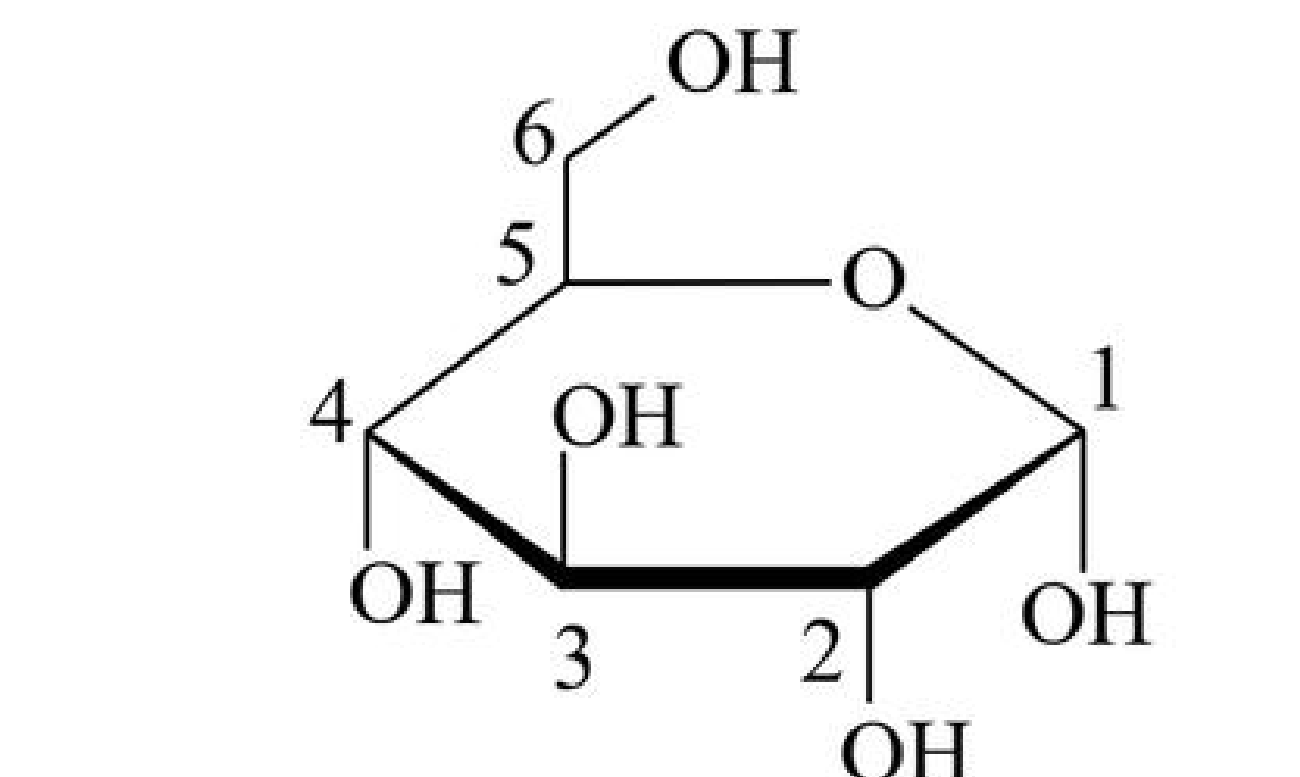
\includegraphics[width=3.5cm]{images_crop_de06/cau10_alpha_glucose.png}
\end{minipage}
\loigiai{}
\end{ex}

\begin{ex}
Dung dịch saccharose tinh khiết không có tính khử, nhưng khi đun nóng với dung dịch \ce{H2SO4} lại có thể cho phản ứng tráng gương. Đó là do:
\choice
{Đã có sự tạo thành aldehyde sau phản ứng}
{Saccharose bị thuỷ phân tạo thành glucose và fructose}
{Saccharose bị thuỷ phân tạo thành glucose}
{Saccharose bị thuỷ phân tạo thành fructose}
\loigiai{}
\end{ex}

\begin{ex}
Phát biểu nào sau đây \textbf{sai}?
\choice
{Thủy phân saccharose chỉ thu được glucose}
{Glucose có khả năng tham gia phản ứng tráng bạc}
{Cellulose và tinh bột đều thuộc loại polysaccharide}
{Cellulose có cấu tạo mạch không phân nhánh}
\loigiai{}
\end{ex}

\begin{ex}
(SBT -- CTST). Mạch nha là tên gọi khác của carbohydrate nào sau đây?
\choice
{Glucose}
{Fructose}
{Saccharose}
{Maltose}
\loigiai{}
\end{ex}

\begin{ex}
Polysaccharide X là chất rắn, màu trắng, dạng sợi. Trong bông nõn có gần 98\% chất X. Thủy phân X, thu được monosaccharide Y. Phát biểu nào sau đây đúng?
\choice
{Y có tính chất của alcohol đa chức}
{X có phản ứng tráng bạc}
{Phân tử khối của Y bằng 342}
{X dễ tan trong nước}
\loigiai{}
\end{ex}

\begin{ex}
(SBT -- CTST). Chất nào sau đây \textbf{không} phải polymer sinh học?
\choice
{Tinh bột}
{Cellulose}
{Glucosamine}
{Chitin}
\loigiai{}
\end{ex}

\begin{ex}
Cho các phát biểu sau về ứng dụng và trạng thái tự nhiên của glucose và fructose:\\
(a) Cả glucose và fructose đều là chất rắn, dễ tan trong nước, có vị ngọt.\\
(b) Glucose có nhiều trong quả chín (nhất là nho chín), fructose có nhiều trong mật ong.\\
(c) Dung dịch truyền tĩnh mạch là glucose 5\%.\\
(d) Glucose và fructose chủ yếu đóng vai trò cung cấp năng lượng cho tế bào.\\
Số phát biểu đúng là:
\choice
{3}
{4}
{1}
{2}
\loigiai{}
\end{ex}

\begin{ex}
Cho các phát biểu sau:\\
(a) Glucose được gọi là đường nho do có nhiều trong quả nho chín.\\
(b) Chất béo là diester của glycerol với acid béo.\\
(c) Phân tử amylopectin có cấu trúc mạch phân nhánh.\\
(d) Ở nhiệt độ thường, triolein ở trạng thái rắn.\\
(e) Trong mật ong chứa nhiều fructose.\\
(f) Tinh bột là một trong những lương thực cơ bản của con người.\\
Số phát biểu đúng là:
\choice
{5}
{6}
{3}
{4}
\loigiai{}
\end{ex}

\begin{ex}
(SBT -- CTST). Cho các phát biểu sau về carbohydrate:\\
(a) Saccharose và fructose không phải là đường khử.\\
(b) Amylopectin phân nhánh là do sự xuất hiện của liên kết $\alpha$-1,6-glycoside.\\
(c) Cellulose không phân nhánh do chỉ xuất hiện liên kết $\beta$-1,4-glycoside.\\
(d) Số nhóm -OH trong phân tử saccharose là 8.\\
Số phát biểu đúng là:
\choice
{1}
{2}
{3}
{4}
\loigiai{}
\end{ex}

\Closesolutionfile{ans}

\newpage

\vspace{0.15cm}
\noindent
\textbf{PHẦN II (4,0 điểm -- 4 câu): Câu trắc nghiệm đúng sai.}\\
\textit{Thí sinh trả lời từ câu 1 đến câu 4. Trong mỗi ý a), b), c), d) ở mỗi câu, thí sinh chọn đúng hoặc sai.}

\setcounter{ex}{0}

\begin{ex}
(SBT -- KNTT).
\choiceTF
{Glucose và fructose đều có công thức phân tử là \ce{C6H12O6}}
{Glucose và fructose đều tồn tại dạng mạch hở và mạch vòng}
{Glucose và fructose đều là pentahydroxy aldehyde}
{Dạng vòng của glucose và fructose đều là vòng sáu cạnh}
\loigiai{}
\end{ex}

\begin{ex}
Cấu trúc phân tử saccharose như sau:
{\centering
	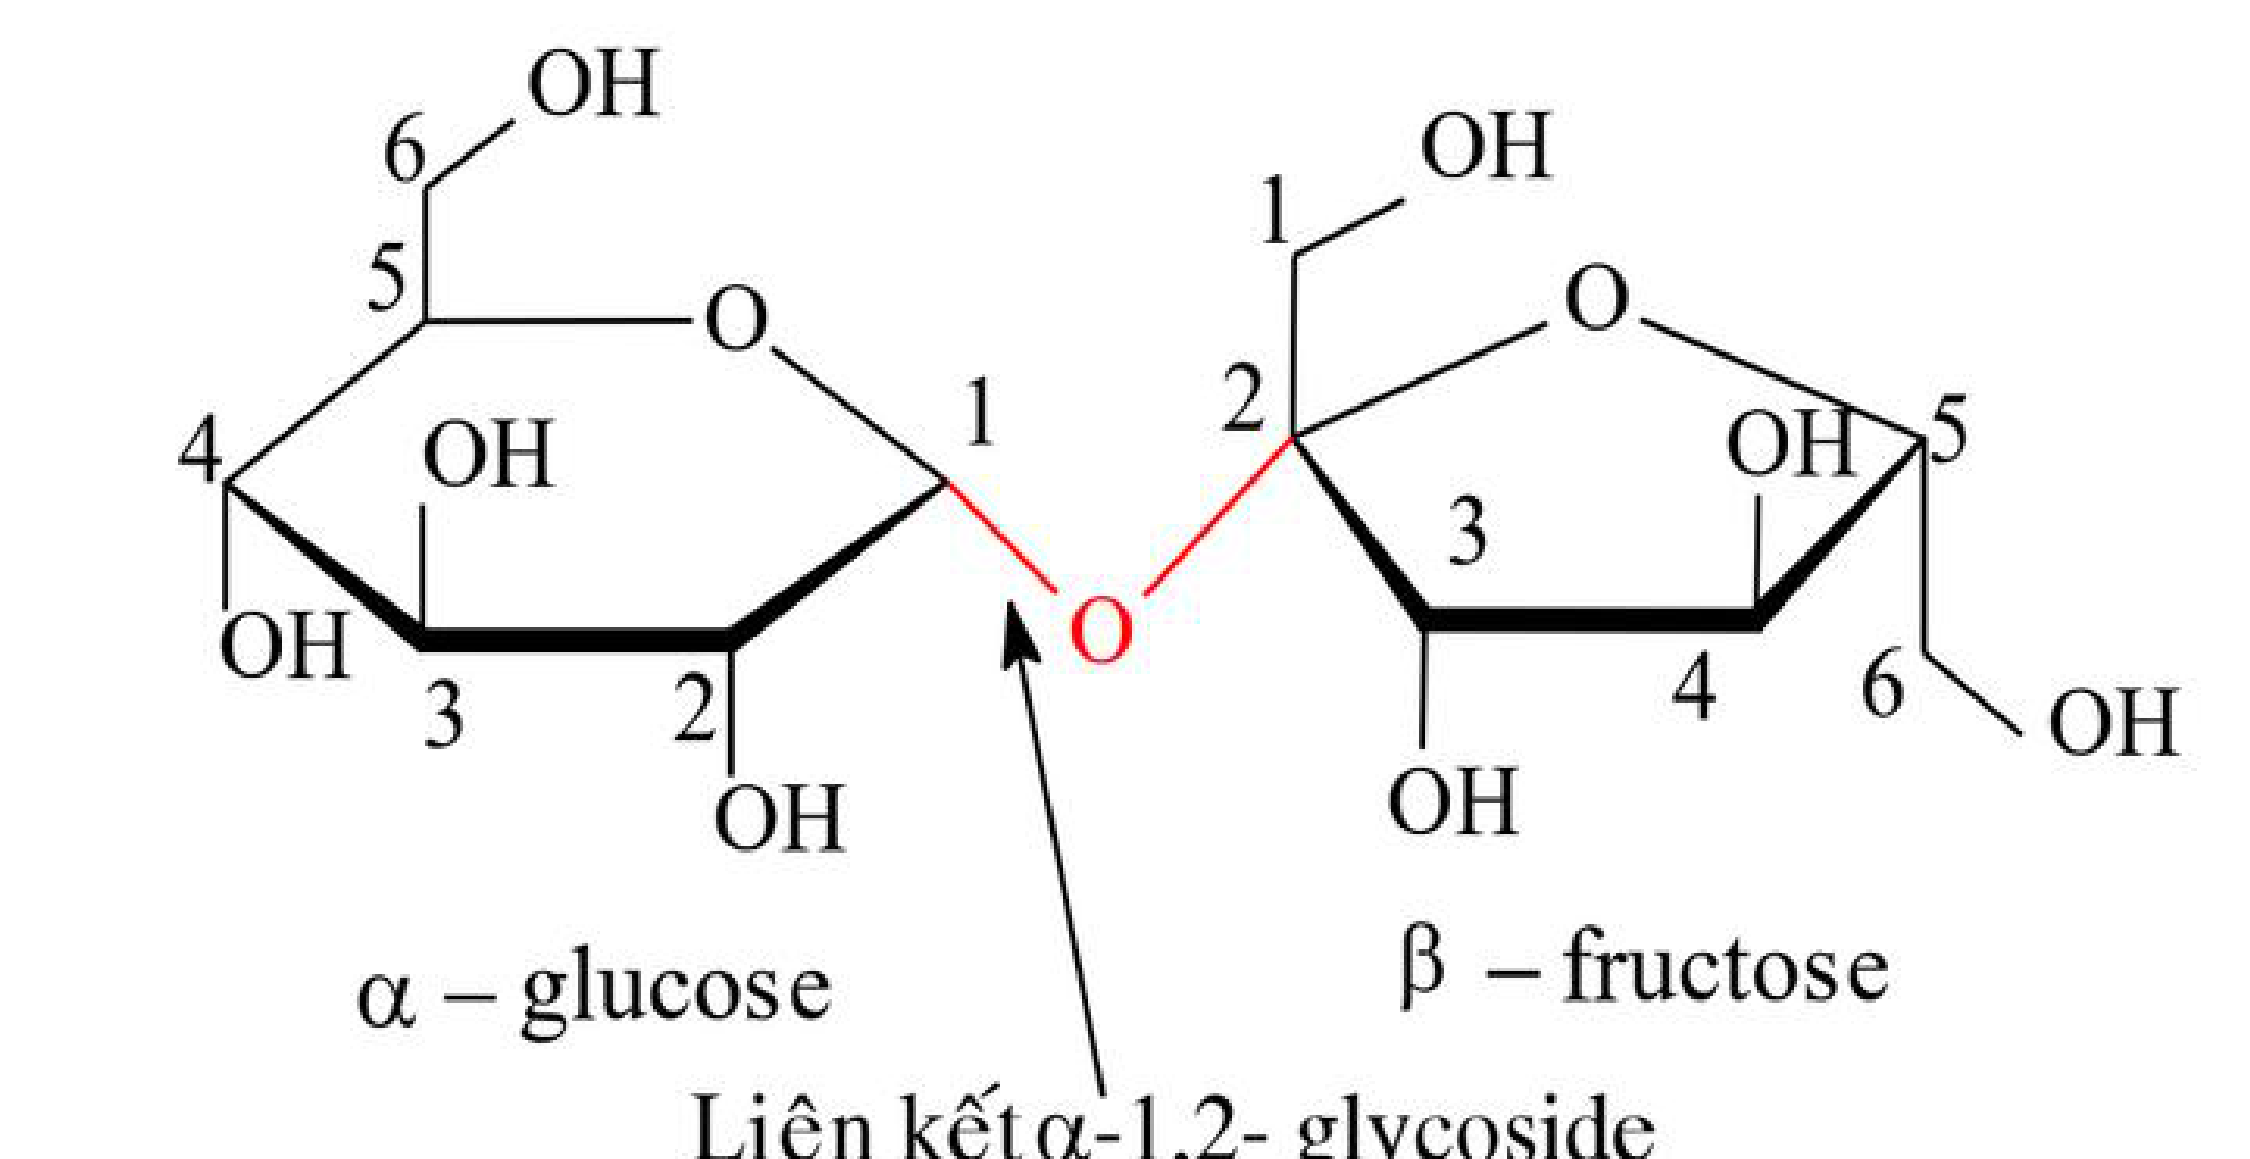
\includegraphics[width=3.6cm]{images_crop_de06/p2_cau2_saccharose.png}\par}
\choiceTF
{Phân tử saccharose gồm một gốc $\alpha$-glucose và một gốc $\beta$-fructose}
{Phân tử saccharose có chứa nhóm -OH hemiacetal}
{Phân tử saccharose có chứa nhóm -OH hemiketal}
{Hai gốc monosaccharide trong saccharose được liên kết với nhau bởi một nguyên tử oxygen}
\loigiai{}
\end{ex}

\begin{ex}
Tiến hành thí nghiệm phản ứng của hồ tinh bột với iodine theo các bước sau đây:\\
\textit{Bước 1:} Cho vài giọt dung dịch iodine vào ống nghiệm đựng sẵn 2 mL dung dịch hồ tinh bột.\\
\textit{Bước 2:} Đun nóng dung dịch một lát, sau đó để nguội.
{\centering
	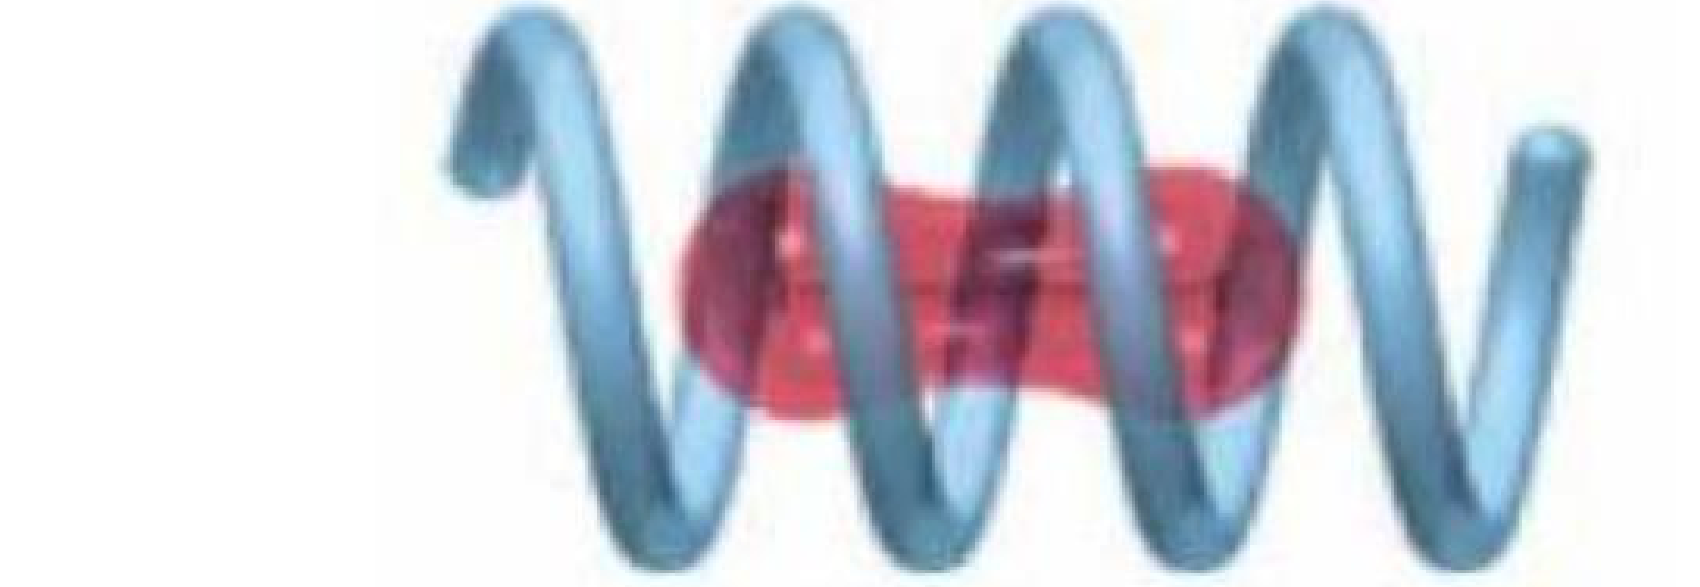
\includegraphics[width=2.5cm]{images_crop_de06/p2_cau3_tinh_bot_iodine.png}\\
	{\footnotesize\itshape\color{hfRed}\textbf{Mô hình tương tác giữa tinh bột \& iodine}}\par}
\choiceTF
{Sau bước 1, dung dịch thu được có màu xanh tím. Sau bước 2, dung dịch bị mất màu}
{Mạch tinh bột xoắn lại tạo các lỗ rỗng, các lỗ rỗng này hấp phụ \ce{I2} tạo nên hợp chất màu xanh tím}
{Nếu nhỏ vài giọt dung dịch iodine lên mặt cắt của quả chuối chín thì màu xanh tím cũng xuất hiện}
{Có thể dùng dung dịch iodine để phân biệt hai dung dịch riêng biệt gồm hồ tinh bột và saccharose}
\loigiai{}
\end{ex}

\begin{ex}
Thí nghiệm phản ứng của cellulose với nitric acid:\\
\textbf{Hoá chất:} cellulose (bông), dung dịch \ce{HNO3} đặc, dung dịch \ce{H2SO4} đặc, dung dịch \ce{NaHCO3} loãng, quỳ tím.\\
\textbf{Dụng cụ:} cốc thuỷ tinh 100 mL, chậu nước nóng, chậu nước đá, đũa thuỷ tinh, giấy lọc, đĩa sứ, đèn cồn.\\
\textbf{Tiến hành:}\\
\textit{Bước 1:} Cho khoảng 5 mL dung dịch \ce{HNO3} đặc vào cốc thuỷ tinh ngâm trong chậu nước đá. Thêm từ từ khoảng 10 mL dung dịch \ce{H2SO4} đặc vào cốc và khuấy đều.\\
\textit{Bước 2:} Lấy cốc ra khỏi chậu nước đá, thêm tiếp một nhúm bông vào cốc và dùng đũa thuỷ tinh ấn bông ngập trong dung dịch. Ngâm cốc trong chậu nước nóng khoảng 10 phút.\\
\textit{Bước 3:} Để nguội, lấy sản phẩm ra khỏi cốc, rửa nhiều lần với nước lạnh (đến khi nước rửa không đổi màu quỳ tím), sau đó rửa lại bằng dung dịch \ce{NaHCO3} loãng. Ép sản phẩm giữa hai miếng giấy lọc và làm khô tự nhiên. Sau đó, để sản phẩm lên đĩa sứ rồi đốt cháy.
{\centering
	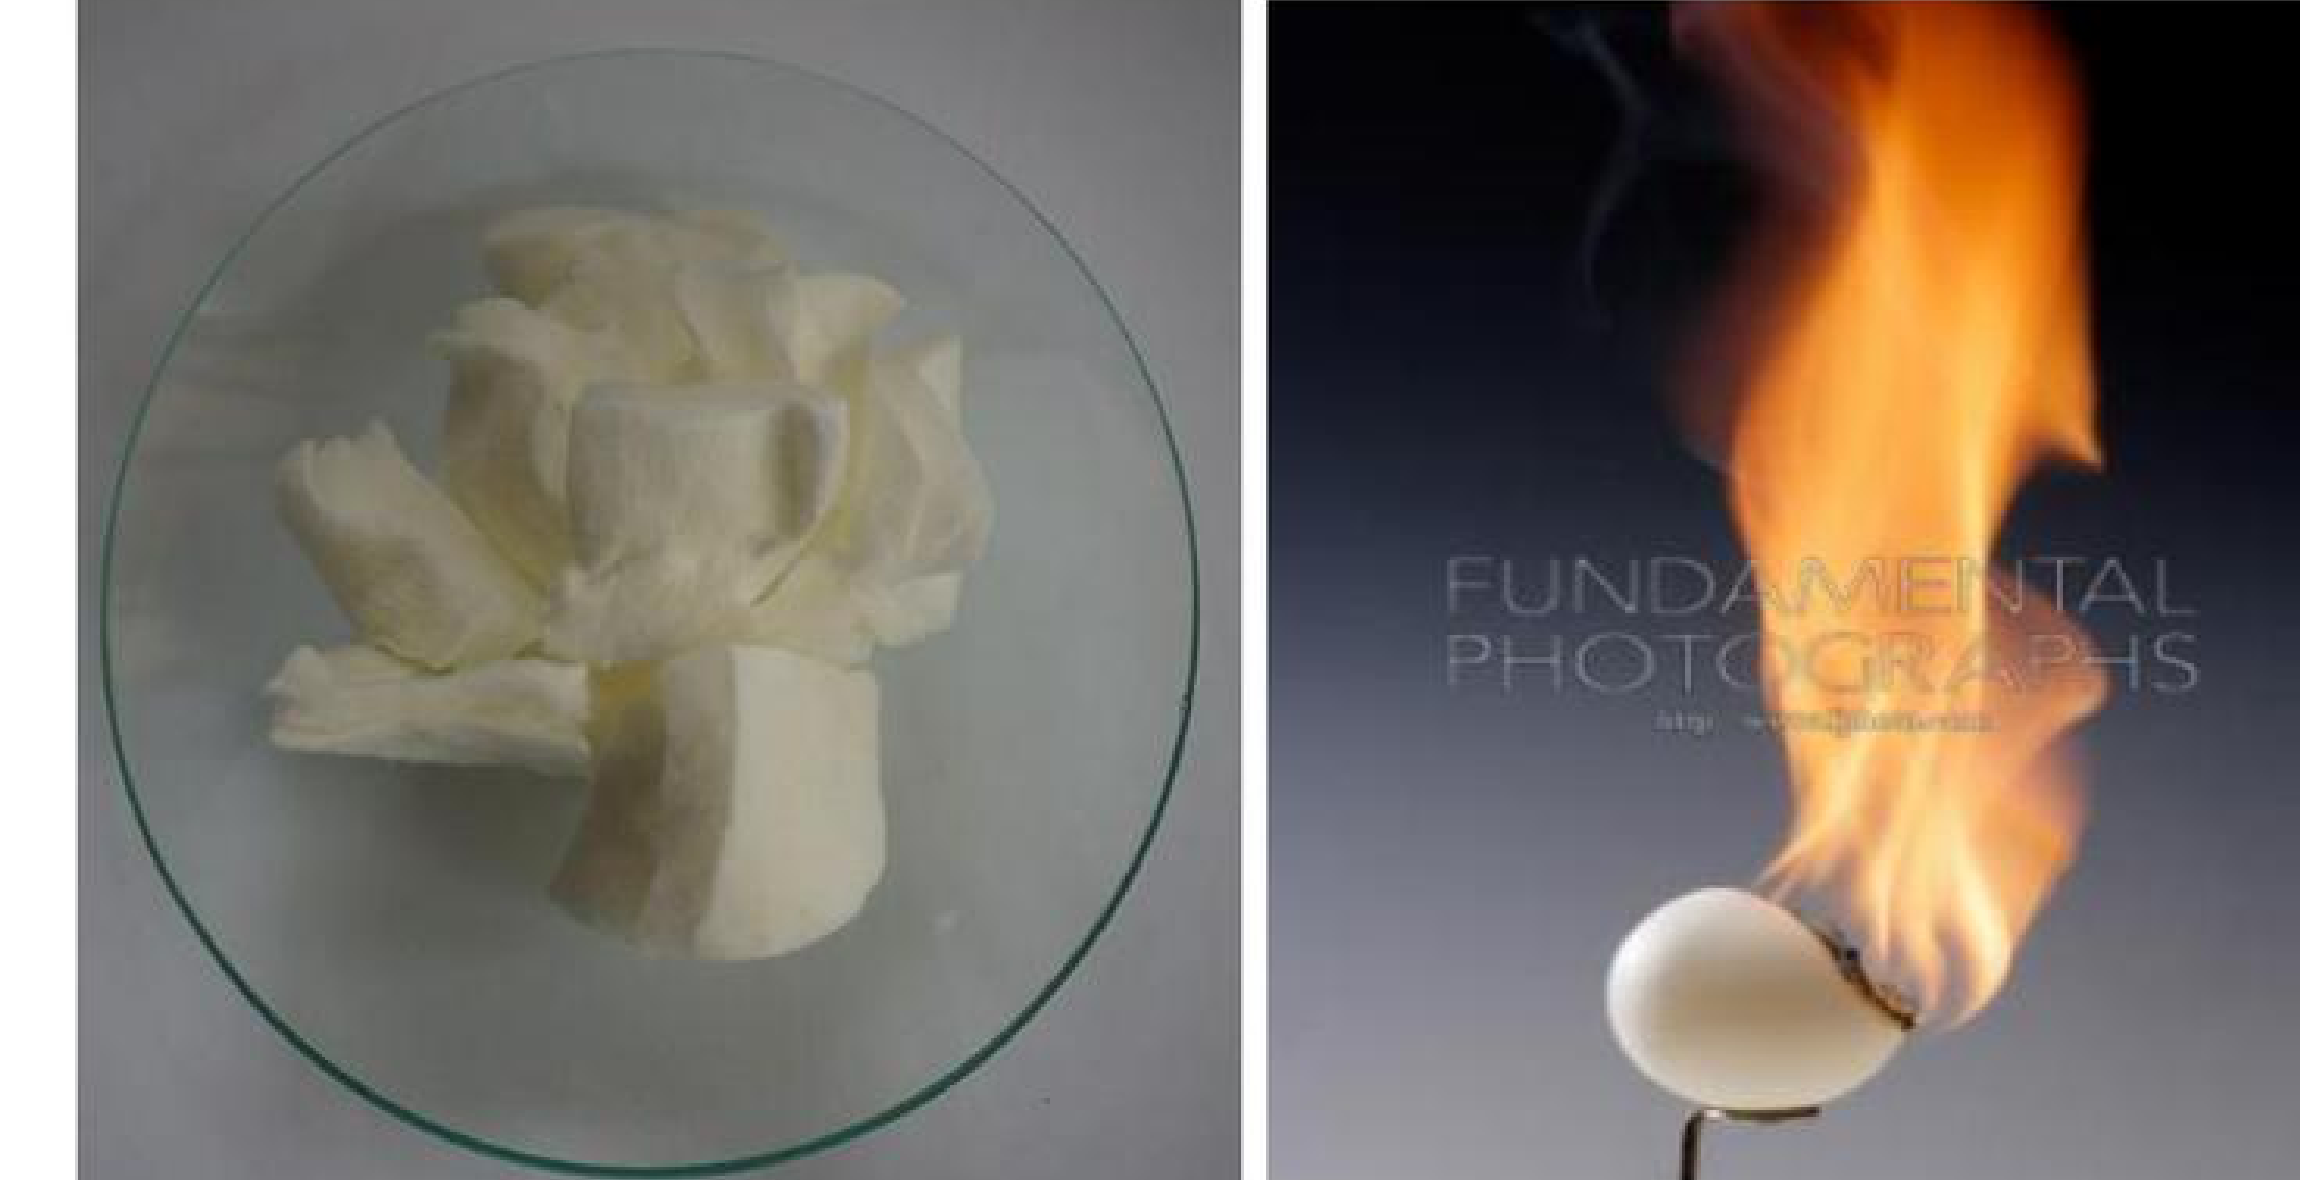
\includegraphics[width=3.6cm]{images_crop_de06/p2_cau4_cellulose_trinitrate.png}\\
	{\footnotesize\itshape\color{hfRed}\textbf{Cellulose trinitrate \qquad\qquad Cellulose trinitrate cháy}}\par}
\choiceTF
{Sau bước 3, sản phẩm thu được có màu vàng}
{Có thể thay thế nhúm bông bằng tinh bột}
{Sau bước 3, lấy sản phẩm thu được đốt cháy thấy có khói trắng xuất hiện}
{Thí nghiệm trên chứng minh mỗi mắt xích trong phân tử cellulose có 3 nhóm OH tự do}
\loigiai{}
\end{ex}

\newpage

\vspace{0.15cm}
\noindent
\textbf{PHẦN III (1,5 điểm -- 6 câu): Câu trắc nghiệm yêu cầu trả lời ngắn.}\\
\textit{Thí sinh trả lời từ câu 1 đến câu 6. Mỗi câu hỏi thí sinh điền câu trả lời vào ô tương ứng.}

\setcounter{ex}{0}

\begin{ex}
Cho các chất: saccharose, glucose, fructose, formic acid và acetic aldehyde. Trong các chất trên, số chất vừa có khả năng tham gia phản ứng tráng bạc vừa có khả năng phản ứng với \ce{Cu(OH)2} ở điều kiện thường là bao nhiêu?
\loigiai{}
\noindent\textbf{Đáp số:} \dotfill
\end{ex}

\begin{ex}
\begin{minipage}{0.65\textwidth}
Phân tử maltose ở dạng mạch vòng (hình bên) có bao nhiêu nhóm alcohol bậc 2?
\loigiai{}
\noindent\textbf{Đáp số:} \dotfill
\end{minipage}\hfill
\begin{minipage}{0.33\textwidth}
\centering
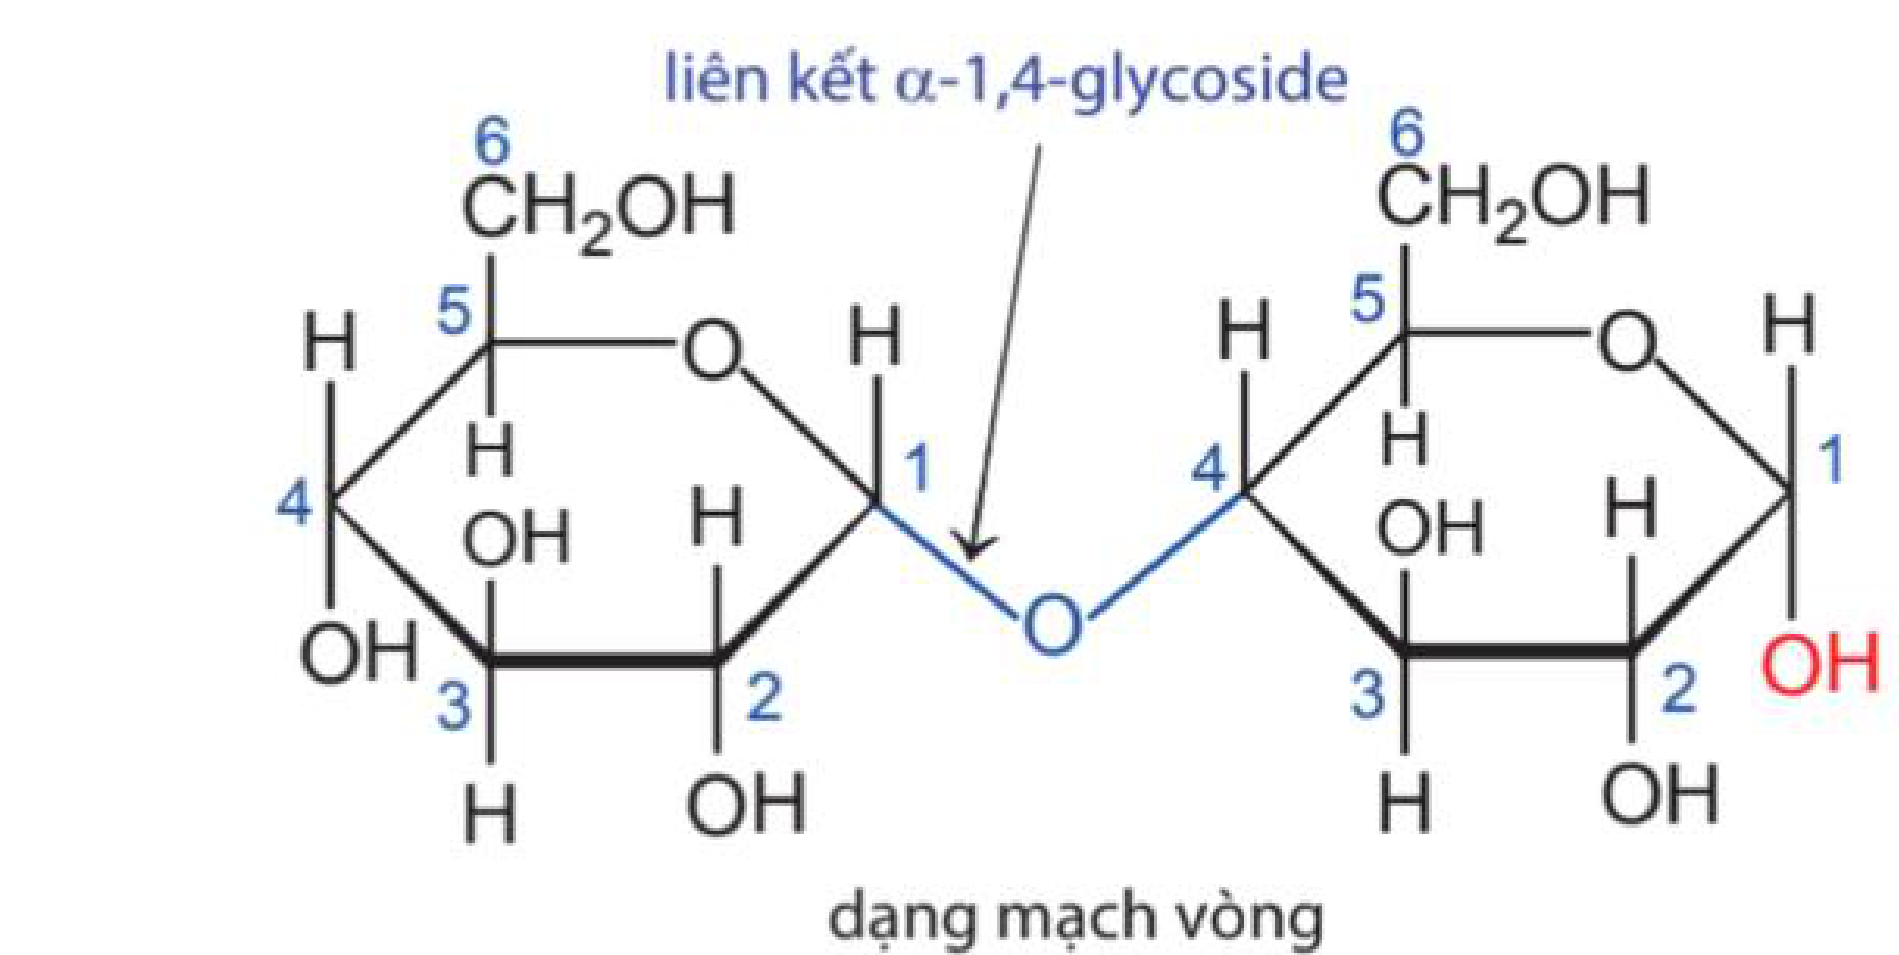
\includegraphics[width=4.8cm]{images_crop_de06/p3_cau2_maltose.png}
\end{minipage}
\end{ex}

\begin{ex}
Cho các phản ứng sau: hoà tan \ce{Cu(OH)2} ở nhiệt độ thường tạo dung dịch xanh lam, phản ứng với thuốc thử Tollens, \ce{Cu(OH)2}/\ce{OH^-} ($t^\circ$), thủy phân môi trường acid, phản ứng màu với dung dịch iodine, phản ứng với \ce{HNO3} đặc/\ce{H2SO4} đặc ($t^\circ$). Số phản ứng mà cellulose có khả năng tham gia phản ứng là
\loigiai{}
\noindent\textbf{Đáp số:} \dotfill
\end{ex}

\begin{ex}
Trong y học, glucose làm thuốc tăng lực cho người bệnh, dễ hấp thu và cung cấp khá nhiều năng lượng. Phản ứng oxi hóa glucose tạo thành \ce{CO2} và \ce{H2O} cung cấp năng lượng cho cơ thể. Một người bệnh được truyền hai chai chứa 250 mL dung dịch glucose 5\%. Tính năng lượng tối đa bệnh nhân nhận được từ các chai truyền glucose đó. Biết nhiệt tạo thành của glucose \ce{C6H12O6}, \ce{CO2} và \ce{H2O} lần lượt là $-1\,271\text{ kJ/mol}$, $-393{,}5\text{ kJ/mol}$ và $-285{,}8\text{ kJ/mol}$; dung dịch glucose 5\% có khối lượng riêng là $1{,}019\text{ g/mL}$. (Làm tròn kết quả đến hàng đơn vị).
\loigiai{}
\noindent\textbf{Đáp số:} \dotfill
\end{ex}

\begin{ex}
Trong công nghiệp, saccharose là nguyên liệu để thủy phân thành glucose và fructose dùng trong kĩ thuật tráng gương, ruột phích. Để thu được 30 kg glucose cần thuỷ phân $m\text{ kg}$ saccharose với hiệu suất phản ứng là 60\%. Giá trị của $m$ là
\loigiai{}
\noindent\textbf{Đáp số:} \dotfill
\end{ex}

\begin{ex}
Một người nông dân có 5 sào ruộng để cấy lúa (3 sào lấy thóc dùng làm thức ăn và 2 sào dùng nấu rượu (ethyl alcohol). Biết năng suất của mỗi sào lúa là $180\text{ kg/sào}$ và một năm thu hoạch 2 vụ. Hàm lượng tinh bột trong gạo là 70\%, biết $1\text{ kg}$ thóc sau khi xát sẽ thu được $0{,}7\text{ kg}$ gạo, ethyl alcohol được nấu là $30^\circ$ với hiệu suất đạt 75\% (khối lượng riêng của ethyl alcohol $D = 0{,}8\text{ g/mL}$). Nếu được bán với giá $20.000\text{ đồng/lít}$ thì số tiền thu được từ việc bán rượu (ethyl alcohol) trong một năm của người nông dân là $a\text{ triệu đồng}$ (làm tròn một chữ số thập phân). Tính $a$.
\loigiai{}
\noindent\textbf{Đáp số:} \dotfill
\end{ex}


\par\vspace{0.1cm}
\centerline{\textbf{---------- HẾT ----------}}

\end{document}
